\section{FIM and CRLB}

The derivation for the FIM is included in the appendix. Given equation 1 let the loglikihood be

\begin{align*}
\log L(\mathbb{\theta}) &= \sum_{i=1}^{N} \log \left[ \alpha \binom{n}{k_1(i)} p^{k_1(i)} (1-p)^{n - k_1(i)} + (1-\alpha) \binom{n}{k_1(i)} q^{k_1(i)} (1-q)^{n - k_1(i)}  \right] 
\end{align*}

Then it follows that the Fisher Information Matrix and the Cramer-Rao Lower Bound are

\begin{align*}
FIM &= -\mathrm{E} \left[\frac{d^2 \log p}{d^2\mathbb{\theta}}\right] \\
CRLB &= FIM^{-1} \\
\end{align*}

The derivations for the derivatives are included in the appendix. When doing the derivations we define

\begin{align*}
P(k | p, n) &= \binom{n}{k}p^{k}(1 - p)^{n - k} \\
P'(k | p, n) &= \frac{dP}{dp} = \binom{n}{k}\left[kp^{k - 1}(1 - p)^{n - k} + (n - k)p^{k}(1 - p)^{n - k - 1}\right]\\
P"(k | p, n) &= \frac{d^2P}{dp^2} = \binom{n}{k}\left[k(k - 1)p^{k - 2}(1 - p)^{n - k} - (-k + n - 1)(n - k)p^k(1 - p)^{-k + n - 2} \right]\\
\end{align*}

The Fisher information matrix is then:

\begin{align*}
-E\begin{bmatrix}\frac{\delta^2\log(L(\mathbb{\theta})}{{\delta\theta}^2}\end{bmatrix} &= -N * E\begin{bmatrix}
F_{\alpha\alpha} F_{\alpha p} F_{\alpha q} \\
F_{\alpha p} F_{pp} F_{pq} \\
F_{\alpha q} F_{pq} F_{qq} \\
\end{bmatrix}
\end{align*}

Where

\begin{align*}
F_{\alpha\alpha} &= \frac{\partial^2L(\mathbb{\theta})}{\partial\alpha^2} = \frac{(P(k | p, n) - P(k | q, n))^2}{(\alpha P(k | p, n) + (1 - \alpha) P(k | q, n))^2} \\
F_{\alpha p} &= \frac{\partial^2L(\mathbb{\theta})}{\partial\alpha\partial p} = \frac{P'(k | p, n)P(k | q, n)}{(\alpha P(k | p, n) + (1 - \alpha) P(k | q, n))^2} \\
F_{\alpha q} &= \frac{\partial^2L(\mathbb{\theta})}{\partial\alpha\partial q} = \frac{-P(k | p, n)P'(k | q, n)}{(\alpha P(k | p, n) + (1 - \alpha) P(k | q, n))^2} \\
F_{pp} &= \frac{\partial^2L(\mathbb{\theta})}{\partial p^2} = \frac{\alpha^2P"(k | p, n)P(k | p, n) + \alpha(1 - \alpha)P"(k | p, n)P(k | q, n) - \alpha^2P(k | p, n)^2}{(\alpha P(k | p, n) + (1 - \alpha) P(k | q, n))^2} \\
F_{pq} &= \frac{\partial^2L(\mathbb{\theta})}{\partial p\partial q} = \frac{-\alpha(1 - \alpha)P'(k | p, n)P'(k | p, n)}{(\alpha P(k | p, n) + (1 - \alpha) P(k | q, n))^2} \\
F_{qq} &= \frac{\partial^2L(\mathbb{\theta})}{\partial q^2} = \frac{\alpha(1 - \alpha)P"(k | q, n)P(k | p, n) + (1 - \alpha)^2P"(k | q, n)P(k | q, n) - (1 - \alpha)^2P'(k | q, n)^2}{(\alpha P(k | p, n) + (1 - \alpha) P(k | q, n))^2}
\end{align*}


A plot for the CRLB is shown below for $\alpha$ = 0.1 ... 0.9, p = 0.2, q = 0.4. As you can see, the theoretical upper bound on the mean squared error increases for both b and q when they are sampled at a small rate. Furthermore, you can see that the mean square error increases for $\alpha$ when $\alpha$ is close to 0.4.

\begin{figure}[!htbp]
	\centering
	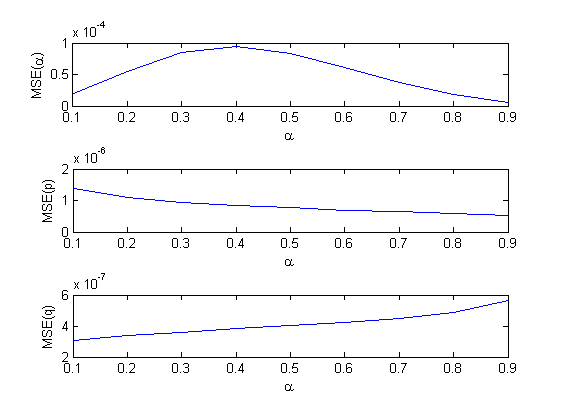
\includegraphics[width=\columnwidth]{images/crlb1.png} %height=1.7in,
	\vspace{-1pt}
	\caption{CRLB for different values of $\alpha$ when p = 0.2, q = 0.4}
	\vspace{-2pt}
	\label{figure:crlb}
\end{figure}

